\documentclass[11pt]{article}
\usepackage[utf8]{inputenc}
\usepackage{fourier}
\usepackage[T1]{fontenc}
\usepackage{natbib}
\usepackage[top=2.7cm, bottom=2.7cm, left=2.5cm, right=2.5cm]{geometry}
\usepackage{graphicx}
\usepackage{authblk}
\usepackage{hyperref}
\usepackage{fancyref}
\setlength\parindent{0pt}

\sloppy

\title{\textbf{Machine Learning and Data Mining with Apache Spark}}
\author{Benjamin Fovet, Maxime Gasque, François Horel, Héloïse Hourquebie, Abderrahman Lahjouji, Anass Seddiki}
\affil{\texttt{\{bfovet, mgasque, fhorel, hhourquebie, alahjouji, aseddiki\} @enseirb-matmeca.fr}}
\date{}

\begin{document}

\maketitle

\textbf{Abstract.} This paper deals with the concepts of \textbf{\textit{machine learning}} and \textbf{\textit{data mining}} social networks, which are increasingly useful for businesses to know the consumers' sentiment towards their brand. This project, intended for use by engineers at Orange France, focuses on the development of a micro-services architecture built around the open source cluster computing framework Apache Spark. Thanks to is distributed model, Spark can process massive amounts of data stored in databases as well as real time data streamed from social networks such as Twitter, Facebook and Orange forum websites. These data are then stored in a cluster database and exposed by an Application Programming Interface (API) server for users to see them in real time.


\section{Context}
% What is Big Data ? (short intro)

Big data is a term used to designate data that is not only too voluminous to fit in a standard database, but is also too diverse and appears at such speed that it cannot be processed using mainstream systems. [Big data now, 2012 edition]
\vskip 9pt
% Orange wants to use Apache Spark
Currently, Orange France is a company already working on big data applications and is interested in using emerging big data technologies. More precisely, among those technologies available today, Apache Spark is the most promising one thanks to its processing performances that makes it well suited to machine learning algorithms.

% What is Apache Spark ? What are the possibilities ? How does it work ?
\subsection{Apache Spark}
\label{apache spark}
Apache Spark is a distributed and highly scalable system, providing the ability to develop applications using languages like Java, Scala (the language used to write Spark itself), Python and R. It was originally developed at the University of California, Berkeley and donated to the Apache Software Foundation in 2013.
Contrary to existing distributed computing software for processing very large data sets, such as Apache Hadoop, Spark is based on an in-memory programming model instead of using the MapReduce [https://wiki.apache.org/hadoop/MapReduce] disk-based model, allowing it to be faster and more flexible. For instance, Spark can sort 100 TB of data three times faster and with ten times fewer machine than MapReduce [https://spark.apache.org/news/spark-wins-daytona-gray-sort-100tb-benchmark.html].

\newpage
Spark consists of four main interoperable components. The figure \ref{spark-stack} below shows the modules built on top of the Spark Core.

\begin{figure}[h!]
    \centering
    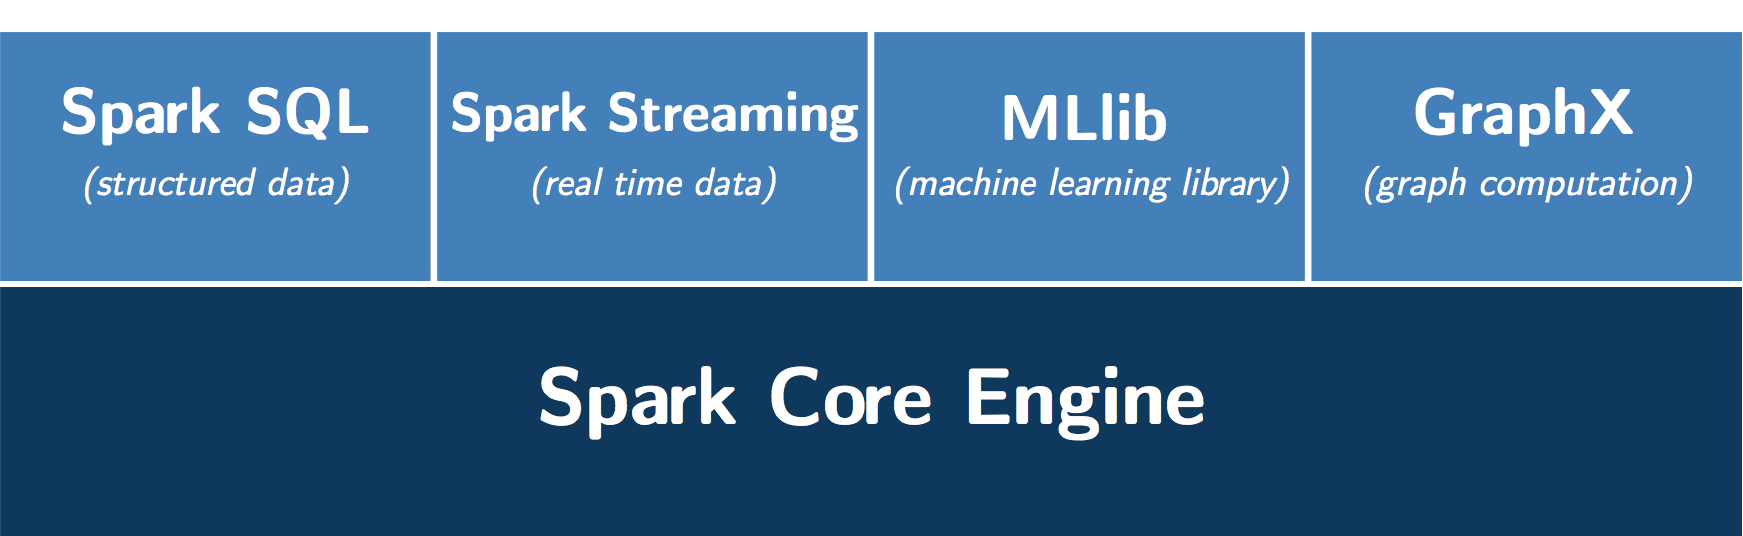
\includegraphics[scale=0.22]{img/spark-stack.eps}
    \caption{The Spark stack}
    \label{spark-stack}
\end{figure}

Spark Core is the foundation of the Spark project and contains features such as task scheduling, memory management, fault recovery and more. On top of that lies four modules.
Spark SQL is Spark's package for working with structured data which allows SQL queries on many sources of data.
Spark Streaming leverages Spark Core capabilities to enable processing of live streams of data. It is used extensively in this project for fetching data from social networks.
MLlib is a library containing machine learning algorithms that can be applied to compute statistical models from data.
Finally, GraphX is another library for manipulating graphs and performing graph computations. 

% Our goal is to demonstrate Spark capabilities, effectiveness and usability through use cases
\subsection{Using Spark in real world scenarios}
The goal of this project is to demonstrate Spark capabilities, effectiveness and usability. At first, requirements were not clearly defined as this project is mainly aimed at exploring what can be done with Spark, but they had to match certain expectations from Orange. These requirements, introduced in the next section, take the shape of use cases as well as Spark integration with other tools.

\section{Developed use cases}
% Video use case
\subsection{Estimating the crowd in Orange stores}

In the way Google shows rush hours of stores and businesses [https://support.google.com/business/answer/6263531?hl=en], the first use case consists of analyzing videos to deduce when customers are more likely to visit Orange stores.

% Social networks use case
\subsection{Data mining social networks}

\subsubsection{Identifying useful sources}

Social networks are a highly valuable source of information about consumers relationship towards a brand. For instance, Orange uses Facebook through two pages: \href{https://www.facebook.com/Orange.France/?ref=ts}{\textbf{Orange}} and \href{https://www.facebook.com/sosh/?fref=ts}{\textbf{Sosh}}, manages several Twitter accounts: \href{https://twitter.com/orange}{\textbf{@orange}} and \href{https://twitter.com/Orange_France}{\textbf{@Orange\_France}} for general communication about Orange, \href{https://twitter.com/Sosh_fr}{\textbf{@Sosh\_fr}} and \href{https://twitter.com/Orange_conseil}{\textbf{@Orange\_conseil}} as after-sales service accounts. Moreover, consumers can access forums at \href{https://communaute.orange.fr}{\url{communaute.orange.fr}}.

All these sources are used for fetching live data and feeding Spark with them.

\subsubsection{Spark applications}

As said in section~\ref{apache spark}, Spark applications can be written in several languages: Java, Python or Scala. Scala was initially chosen since Spark itself is developed in Scala and it is also less verbose than Java code. Furthermore, Java and Scala applications have the advantage of being compiled and packaged into an \textbf{Uber-JAR}. JAR (Java ARchive) is a package file format used to aggregate class files required for an application to run, and an Uber-JAR is a JAR that not only contains the application code but also embeds its dependencies as well. This way, the application only needs to be submitted with the Uber-JAR file to Spark to be executed.

Applications are also separated by sources, allowing a more flexible development and release to production as well as a reduction of risks. Indeed, Facebook and Twitter have their own independent API services and having issues with one will not impact the other. This structure also leads to a better bug tracking management with having the bug-free application uninterrupted.

\subsubsection{Sentiment analysis}

Sentiment analysis refers to the use of natural language processing and text analysis to identify and extract subjective information in source materials. It aims to classify the polarity of a given text — whether the expressed opinion is positive, negative, or neutral. 
Based on the source, sentiment analysis is applied to tweets on Twitter, posts on Facebook, and thread titles and messages on forums.

\paragraph{Dictionary-based approach}

The first approach consists of deciding whether a text is positive, negative or neutral by looking at words in isolation, giving positive points for positive words and negative points for negative words found in two separate dictionaries and then summing up these points.

The following workflow example is based on a real tweet from an Orange consumer.

\begin{figure}[h!]
    \centering
    
\includegraphics[scale=0.6]{img/tweet1.png}
    \caption{Tweet from a user to \textbf{@Orange\_conseil}}
    \label{tweet1}
\end{figure}

The first step is to tokenize the text, translating a sentence into a list of independant words. This is done using the \texttt{FrenchTokenizer} \url{https://github.com/stanfordnlp/CoreNLP/blob/master/src/edu/stanford/nlp/international/french/process/FrenchTokenizer.java}, part of the Stanford CoreNLP suite of Natural Language Processing tools. Along with tokenizing a text, common words with no interesting meaning such as "le", "dans", "à" also known as "stop words" are filtered out to produce the following list of meaningful words.

\begin{figure}[h!]
    \centering
    connexion, internet, vraiment, instable, moment, souvent, aucun, accès, internet, normal
    \caption{Words after tokenization}
    \label{tokens}
\end{figure}

Next, each word in the above list is looked up in the positive and negative words dictionaries. If found, the weight associated with a negative or positive sentiment, depending on which dictionary the word has been found in, is increased by an increment of one.

In the above tweet, the words \textit{instable, aucun} can be found in the negative words. The word \textit{normal} is not considered positive nor negative because of the context. In order to label it accordingly, a look behind processing has to be implemented to detect the presence of the word \textit{pas}. The structure \textit{pas normal} would then be labeled as negative meanwhile \textit{normal} would be positive.

Finally, the sentiment for the whole tweet is given by computing the difference between the positive weight and the negative weight. A sentiment score equal to 0 is associated with "NEUTRAL", while positive scores are marked as "POSITIVE" and negative scores as "NEGATIVE". Consequently, the example tweet has a negative weight of 2 and a positive weight of 0, labeling it as negative.

This method is far from perfect since it gives a sentiment based on separate words instead of the context of a sentence. The sentiment analysis annotator from Stanford CoreNLP \url{https://stanfordnlp.github.io/CoreNLP} was tested before implementing this technique and although it yields more accurate results based on a large grammar treebank, it is only available for English text analysis.

\paragraph{Machine learning-based approach}

% https://spark.apache.org/docs/latest/mllib-naive-bayes.html
% https://spark.apache.org/docs/latest/mllib-ensembles.html#training

Thanks to Spark's Machine Learning library \textit{MLlib}, classification algorithms can be applied to analyze tweets. In this approach, the Naive Bayes algorithm, a probabilistic classifier based on Bayes' theorem, and the Random Forest algorithm, an ensemble of decision trees for binary and multiclass classification, are implemented through two steps: train and predict.

Training the data requires having a set of tweets already classified by hand, with 1 meaning positive and 0 meaning negative. This data set is then loaded and 80\% of the data is split into training data, used to train the classifier model, while 20\% is split into testing data, used to assess the performance and the accuracy of the trained model.
With these algorithms, 74\% of the 1343 tweets is correctly classified. According to the computed results below, the Random Forest algorithm is slightly more accurate than the Naive Bayes algorithm yet it is less time efficient. % Add detail about trees options ?

\begin{center}
\begin{tabular}{|l|c|c|}
  \hline
  Algorithm & Naive Bayes & Random Forest \\
  \hline
  Accuracy & 74.04\% & 77.39\% \\
  Training duration (ms) & 623 & 14266 \\
  Testing duration (ms) & 13 & 193 \\
  \hline
\end{tabular}
\end{center}

Predicting is then possible by applying the previous trained model.

\subsubsection{Specific computed indicators}

\paragraph{Twitter}

% Number of tweets per second
% After sales sosh_fr and orange_conseil time to respond to a tweet
% Number of retweets for a tweet
% Trending hashtags

\paragraph{Facebook}

\paragraph{Orange forums}

% Scraping web pages:
%   - each subforum first page and check date
%       * thread title, link, date, messages
% Number of topics not responded

% Every component of our architecture
\section{Building a microservices architecture}

% Presentation and schema first

Microservices pattern is an architectural style in which large complex software applications are broken down into a collection of small, independent, loosely coupled processes. This helps upgrading, modifying or changing one service instead of taking down the entire system. As shown in the figure below, this project is composed of several services communicating with each other, which are presented in the next sections.

\begin{figure}[h!]
    \centering
    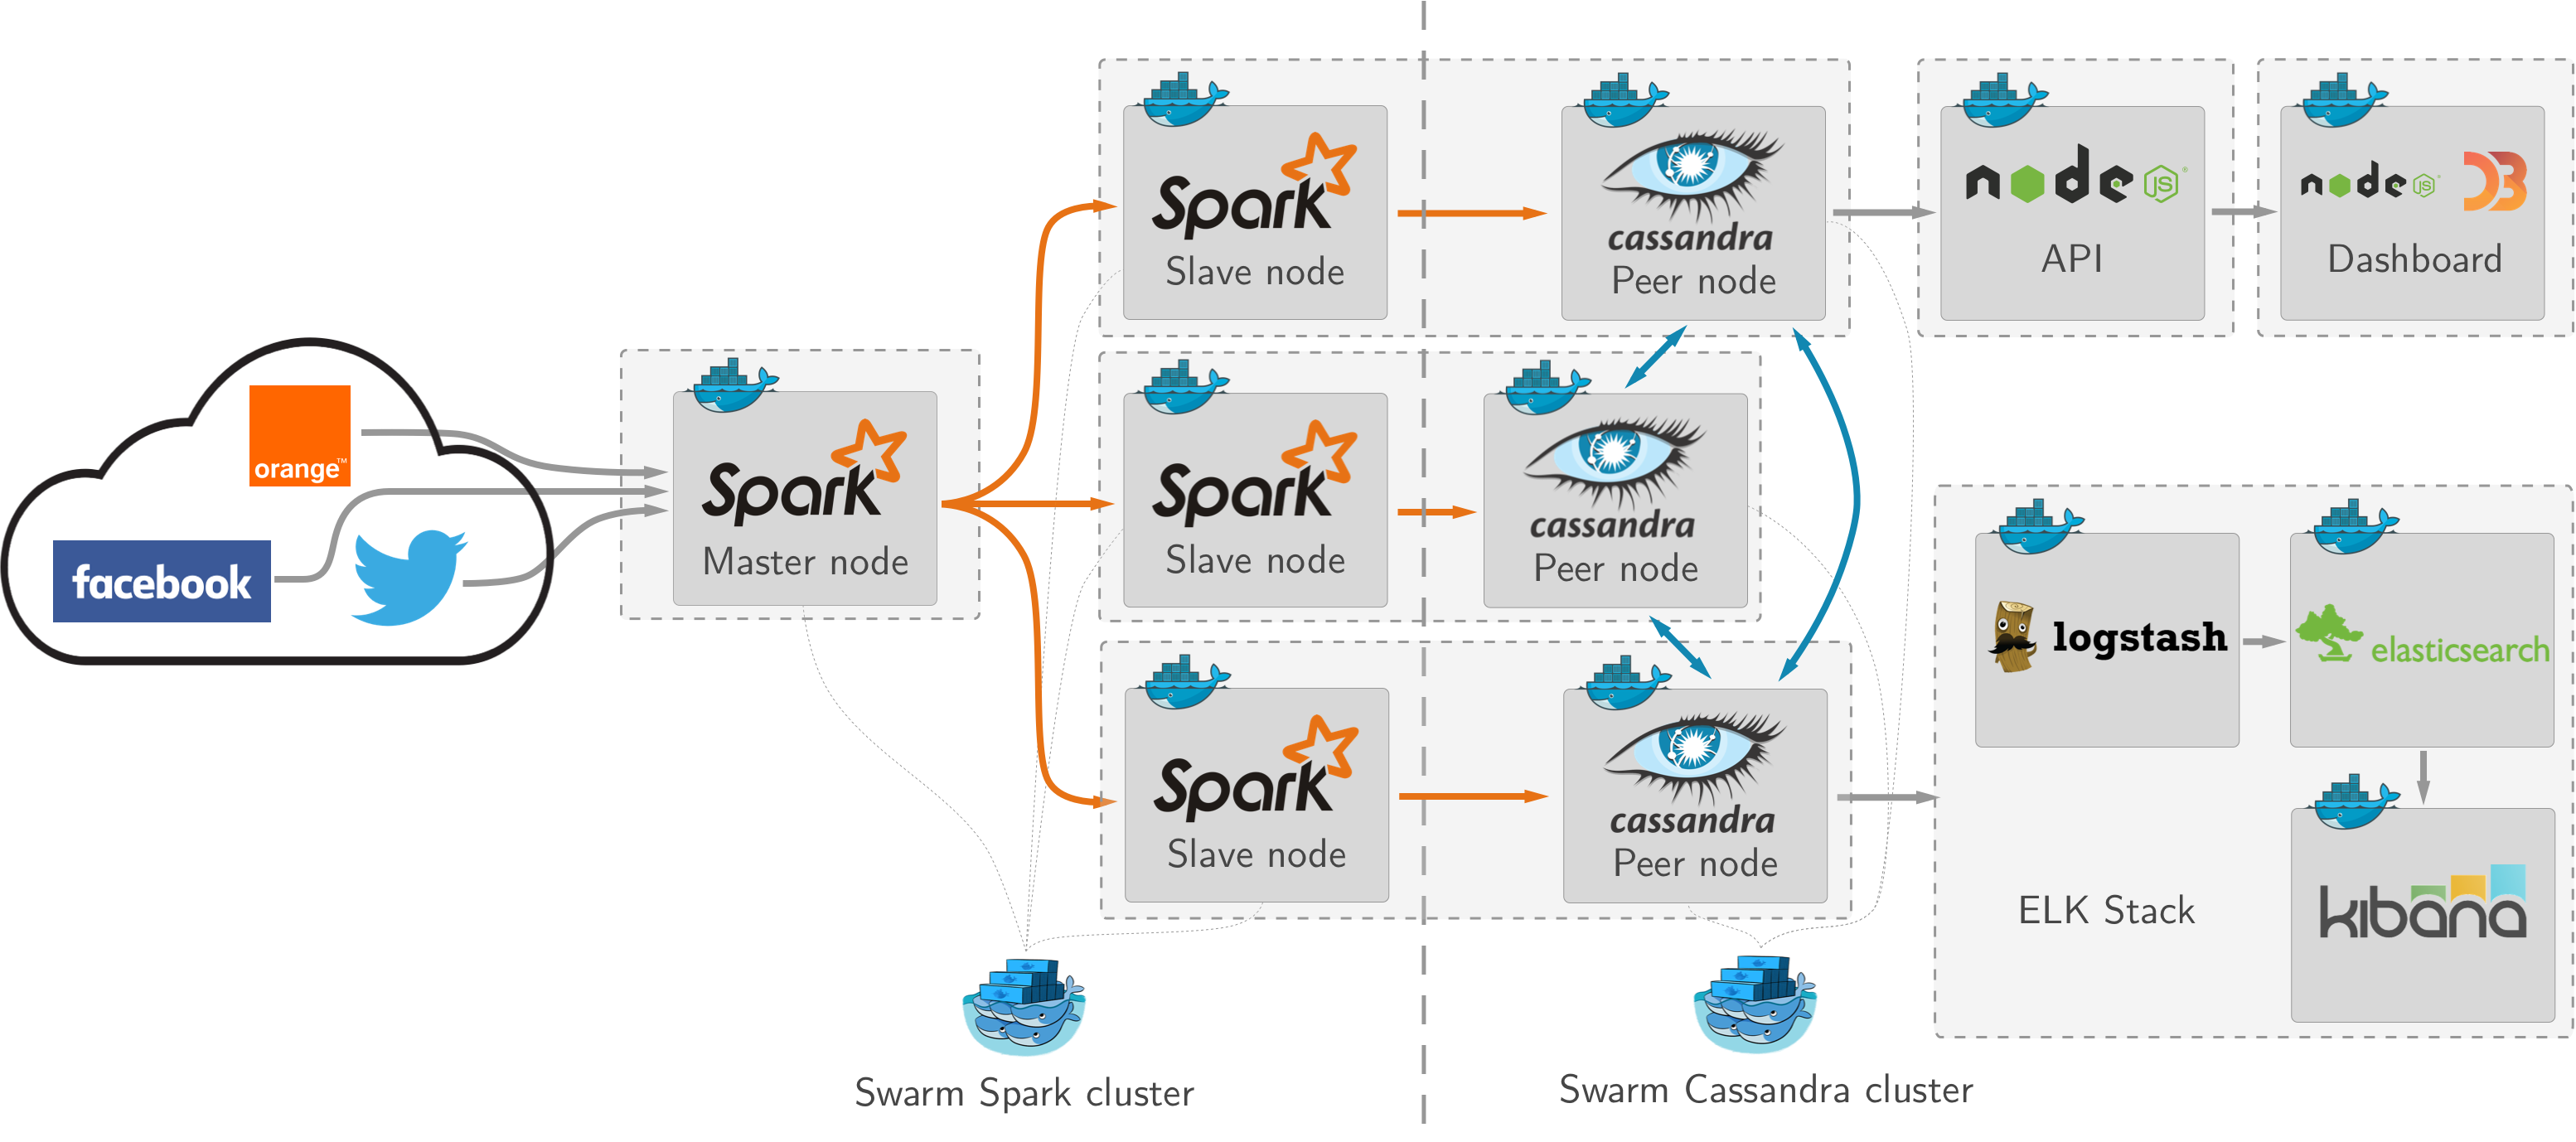
\includegraphics[scale=0.15]{img/archi.png}
    \caption{Deployed infrastructure}
    \label{infra}
\end{figure}

\subsection{Docker}

To facilitate the deployment of each application, Docker is the ideal technology. It automates the deployment of applications inside containers, isolated from the host and other containers by leveraging functionalities of the Linux kernel. Docker containers wrap up a piece of software in a complete filesystem that contains everything it needs to run: code, runtime, system tools, system libraries – ensuring that it will run consistently across all environments. In terms of virtualization, each Docker container uses the host OS (Linux) features instead of requiring an hypervisor and a guest OS like a virtual machine.

\begin{figure}[h!]
    \centering
    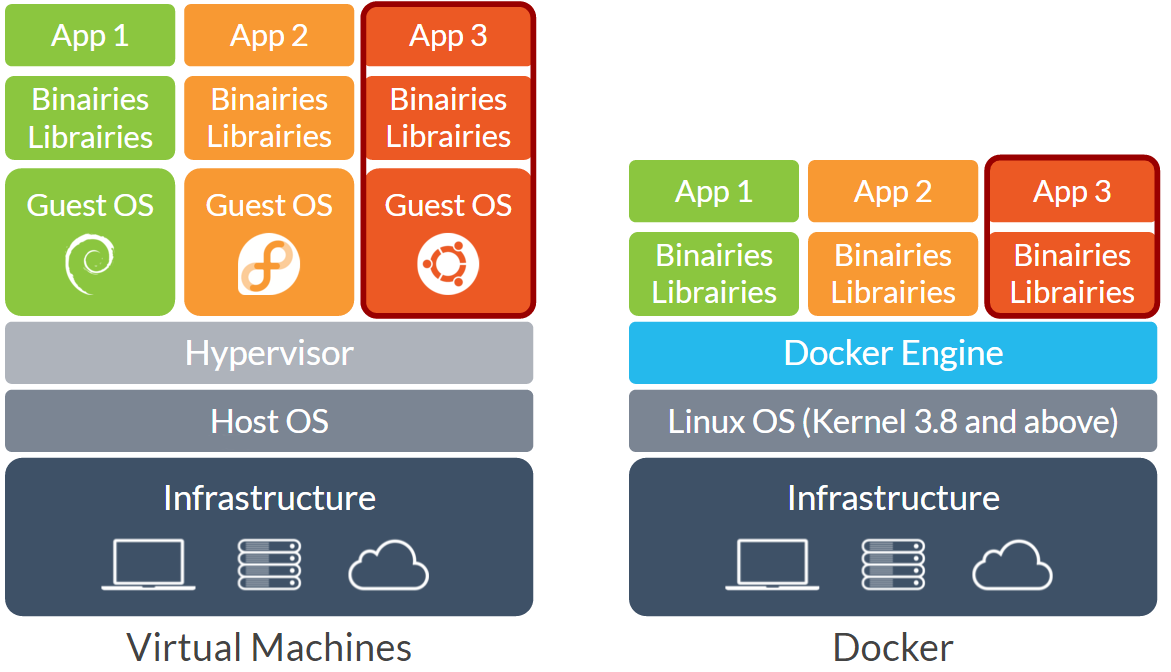
\includegraphics[scale=0.3]{img/docker-vs-vm.png}
    \caption{Comparison between VMs and Docker}
    \label{docker-vs-vm}
\end{figure}

The Spark cluster is deployed with Docker Compose [https://docs.docker.com/compose/] and both clusters are orchestrated with Docker Swarm [https://docs.docker.com/swarm/].

\subsection{Spark cluster}

% https://spark.apache.org/docs/1.6.0/cluster-overview.html
% http://blog.ippon.fr/2014/11/20/utiliser-apache-spark-en-cluster/

Spark is a distributed computing framework, following the master-slave model. It is composed of a master which schedules and shares jobs between one or more workers.

\subsection{Cassandra cluster}

Apache Cassandra is a NoSQL open-source distributed database system. It is designed to handle large amount of data replicated across servers in a cluster. Each node is installed on the same machine as the Spark workers in order to optimize access to the database and minimize network latency.

\paragraph{Parameters}

Ensuring reliability and fault tolerance on multiple nodes is possible by setting the replication factor according to the number of nodes in the cluster. For instance, three nodes (A, B, C) are deployed for this project. 

With a replication factor of 3, the QUORUM level (rounded down to a whole number) is (replication factor/2) + 1 = 2 which means the cluster can tolerate 1 node down. Besides, each node holds 100\% of the data. This allows a client to write data to A and read the exact replica from B.

Furthermore, consistency is configured to use the QUORUM level with the following CQL [\url{http://docs.datastax.com/en/cql/3.1/cql/cql_intro_c.html}] command: CONSISTENCY QUORUM;
With a replication factor of 3, this ensures that 2 nodes are always written and 2 nodes are always read.

\paragraph{Data schema}

Data is stored in different keyspaces related to the aggregated sources: \textit{twitter\_streaming}, \textit{facebook} and \textit{forums} respectively for Twitter, Facebook and Orange forums.

For example, tweets are stored in a table called tweets with extracted fields from Twitter as well as computed ones: response\_time and sentiment.
          
Two other tables are used for storing the velocity in tweets/min (freq) and the most popular hashtags (trends).

\subsection{API}

A RESTful API, developed with NodeJS, is connected to Cassandra to make data available for visualization. 
Its documentation is written with Swagger [http://swagger.io/] for a better representation.

\begin{figure}[h!]
    \centering
    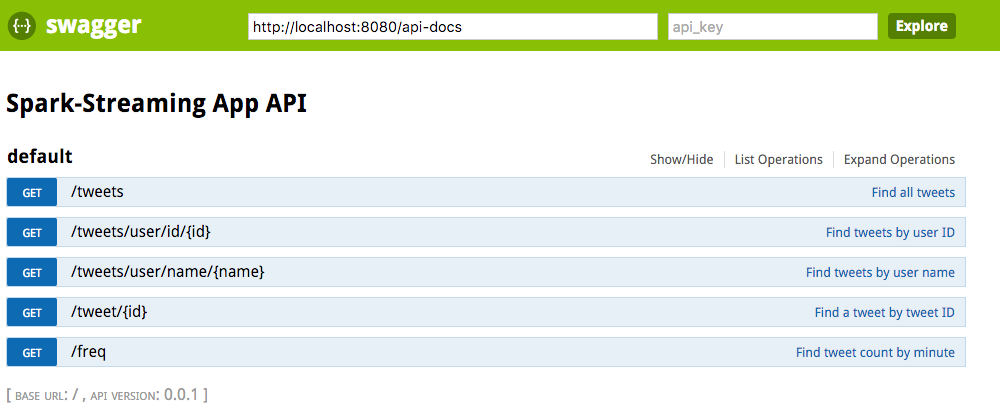
\includegraphics[scale=0.4]{img/api-docs.png}
    \caption{API documentation available at \url{{API_IP_ADDRESS}:8080/docs}}
    \label{socket}
\end{figure}

The NodeJS driver for Cassandra [https://github.com/datastax/nodejs-driver] is implemented for streaming data stored in the database to the API.

Along with this API, another NodeJS web server has been developed to serve a web dashboard, using D3.js for charts. When a client loads the page, data is pushed from the API to the dashboard using socket.io [http://socket.io/]. 

\begin{figure}[h!]
    \centering
    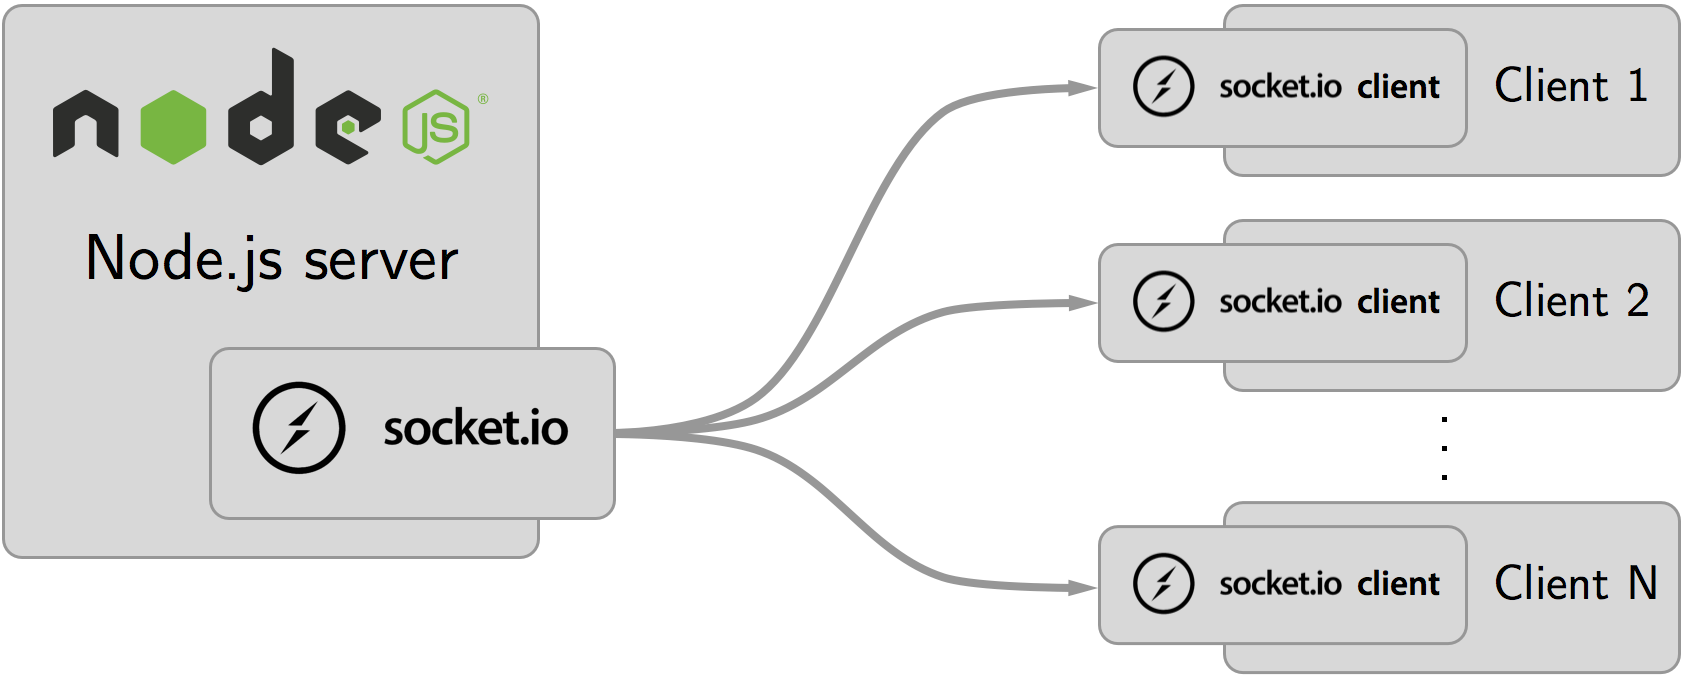
\includegraphics[scale=0.12]{img/api-dashboard-socket.png}
    \caption{Realtime communication between clients and the server with \textbf{socket.io}}
    \label{socket}
\end{figure}


\subsection{ELK stack}

In parallel, the ElasticSearch - Logstash - Kibana stack is tested as a turnkey solution to replace Cassandra, the API server and the web interface. % à détailler

\section{Organization and Management}

\subsection{Methodology}

Agile software methodology was an efficient way of organizing this project where objectives were not accurate and stable at the beginning. The development was split in sprints (or iteration) of 3 weeks (See appendices).
Moreover, short-term sprints allowed a part of the team to stop the video processing development before running low on budget (in hours).

The clients were actively involved in the process and meetings were planned every week when possible to demonstrate and review new features. The progress of the project could be followed thanks to weekly reportings available at \url{bfovet.vvv.enseirb-matmeca.fr/reporting_projet}.

\subsection{Tools}

% GitHub for source code hosting and issue tracking, Trello for sprint planning and task assignment, Google Drive for project documents sharing, Docker Hub for Docker images hosting, Travis-CI for continuous testing, integration and deployment.

\subsection{Issues}

% Data privacy policy: restricted access to Orange data --> alternatives: social networks and open source data sets

% TECHNINCAL ISSUES
% New concept of machine learning
% Many parts to develop and connect together
% New language: scala
% Video processing is time consuming + integration with Spark
% Tuning and configuring spark correctly

\section{Conclusion}

% Spark, useful software for Big Data
%  - Aggregating various sources
%  - Many libraries available for data processing

% Defining stores rush hours
%  - Identifying overcrowded stores
%  - Shortening customers waiting time

% Detecting issues on social networks
%  - Helping community managers focus on unanswered questions
%  - Sentiment towards the brand

% Ouverture sur Apache Flink, next software for Big Data processing, focused on streaming, comparable to Spark Streaming


\section{Bibliography}
\bibliographystyle{plain}
\bibliography{references}

%https://stanfordnlp.github.io/CoreNLP/#citing-stanford-corenlp-in-papers:

Manning, Christopher D., Mihai Surdeanu, John Bauer, Jenny Finkel, Steven J. Bethard, and David McClosky. 2014. The Stanford CoreNLP Natural Language Processing Toolkit In Proceedings of the 52nd Annual Meeting of the Association for Computational Linguistics: System Demonstrations, pp. 55-60. [http://nlp.stanford.edu/pubs/StanfordCoreNlp2014.pdf] [bib]

http://nlp.stanford.edu/publications.shtml:

Richard Socher, Alex Perelygin, Jean Wu, Jason Chuang, Christopher Manning, Andrew Ng, and Christopher Potts. 2013. Recursive Deep Models for Semantic Compositionality Over a Sentiment Treebank. In EMNLP. [pdf, bib, info]

\section{Appendices}
\subsection{Project organization}

\subsubsection{Project planning}
% Gantt chart

\subsubsection{Sprints}
% sprint table with details

%Sprint 0
%    Learning Big Data and Spark
%    Finding the use cases to develop
%Sprint 1
%    Apache Spark deployment 
%    Real-time video processing setup
%    Twitter API exploration
%Sprint 2
%    Twitter mining with Spark
%    Real-time video processing with Spark
%Sprint 3
%    Twitter analysis 
%    Facebook mining & analysis
%    Forums mining & analysis
%    Data visualization


\subsubsection{Burndown chart}


\subsection{Team charter}

\subsection{Data visualization dashboard}


\end{document}